\section{最終の構成と精度}
\label{sec_final}
\subsection{処理の流れ}
図\ref{fig_pipeline}に，最終のアノテーションの処理の流れを示す．
処理は，画像の列挙，生徒による予測，お題文の確認，ラベルの決定の4段階からなる．

\begin{figure}[t]
    \centering
    \begin{tikzpicture}[
        node distance=4mm,
        box/.style={draw, rounded corners=2pt, align=center, font=\footnotesize, minimum width=0.86\linewidth, inner sep=3pt},
        arr/.style={-{Stealth[length=2mm]}, thick}
    ]
        \node[box] (list) {1. 列挙：ハッシュ値が同じ画像をまとめる \\ 6,823,270件 $\to$ 6,609,511枚};
        \node[box, below=of list] (pred) {2. 予測：SigLIP2-so400m の埋め込み $\to$ MLP 3種 \\ ＋ 微調整した SigLIP2-B の確率の平均};
        \node[box, below=of pred] (ver) {3. 確認：お題文と予測した約8\%の画像に \\ Qwen3-VL-8B で確認の質問};
        \node[box, below=of ver] (fin) {4. 決定：確認で偽ならお題文以外で最大の形式 \\ 形式から属性を導き，お題ごとに保存};
        \draw[arr] (list) -- (pred);
        \draw[arr] (pred) -- (ver);
        \draw[arr] (ver) -- (fin);
    \end{tikzpicture}
    \caption{最終のアノテーションの処理の流れ}
    \label{fig_pipeline}
\end{figure}

列挙の段階では，ハッシュ値が同じ画像のうち代表の1枚のみを予測し，結果を同じ内容の全てのお題に展開する．
予測の段階では，各画像を1回だけ読み込み，SigLIP2-so400m の埋め込みと微調整した SigLIP2-B の確率を同時に求める．
埋め込みは保存しておき，ラベルの定義を見直す場合に，教師ラベルを付け直して MLP を学習し直すだけで全件のラベルを更新できるようにした．
確認の段階では，平均した確率で形式がお題文となった画像に限り，Qwen3-VL-8B に確認の質問をする．
決定の段階では，確認の質問の回答が偽の画像を，お題文以外で確率が最大の形式に変え，形式から属性を導く．

\subsection{確認の質問の選択}
教師の構成では，お題文の確認に表\ref{tab_questions}の確認の質問を用いた．
最終の構成の生徒は，2つのモデルの確率の平均によってお題文の誤検出が既に少なく，評価用データでは確認の質問の有無による差がほとんどなかった．
そこで，学習にも評価にも用いていない無作為の2万枚に全ての段階を適用し，確認の質問の働きを直接確かめた．

生徒がお題文と予測した1,615枚のうち，教師と同じ確認の質問はお題文ではないと145枚を答えた．
この145枚を目視で確認したところ，98枚は実際にはお題文であった．
図\ref{fig_o10_wrong}に例を示す．
その多くは，ボケてのテンプレートに投稿者が書いた「こんな〜は嫌だ」のような典型的な題目の句や，主題となる台詞の文であった．
評価用データにはこの種の画像が少ないため，評価用データだけではこの欠点が見えなかった．

\begin{figure*}[t]
    \centering
    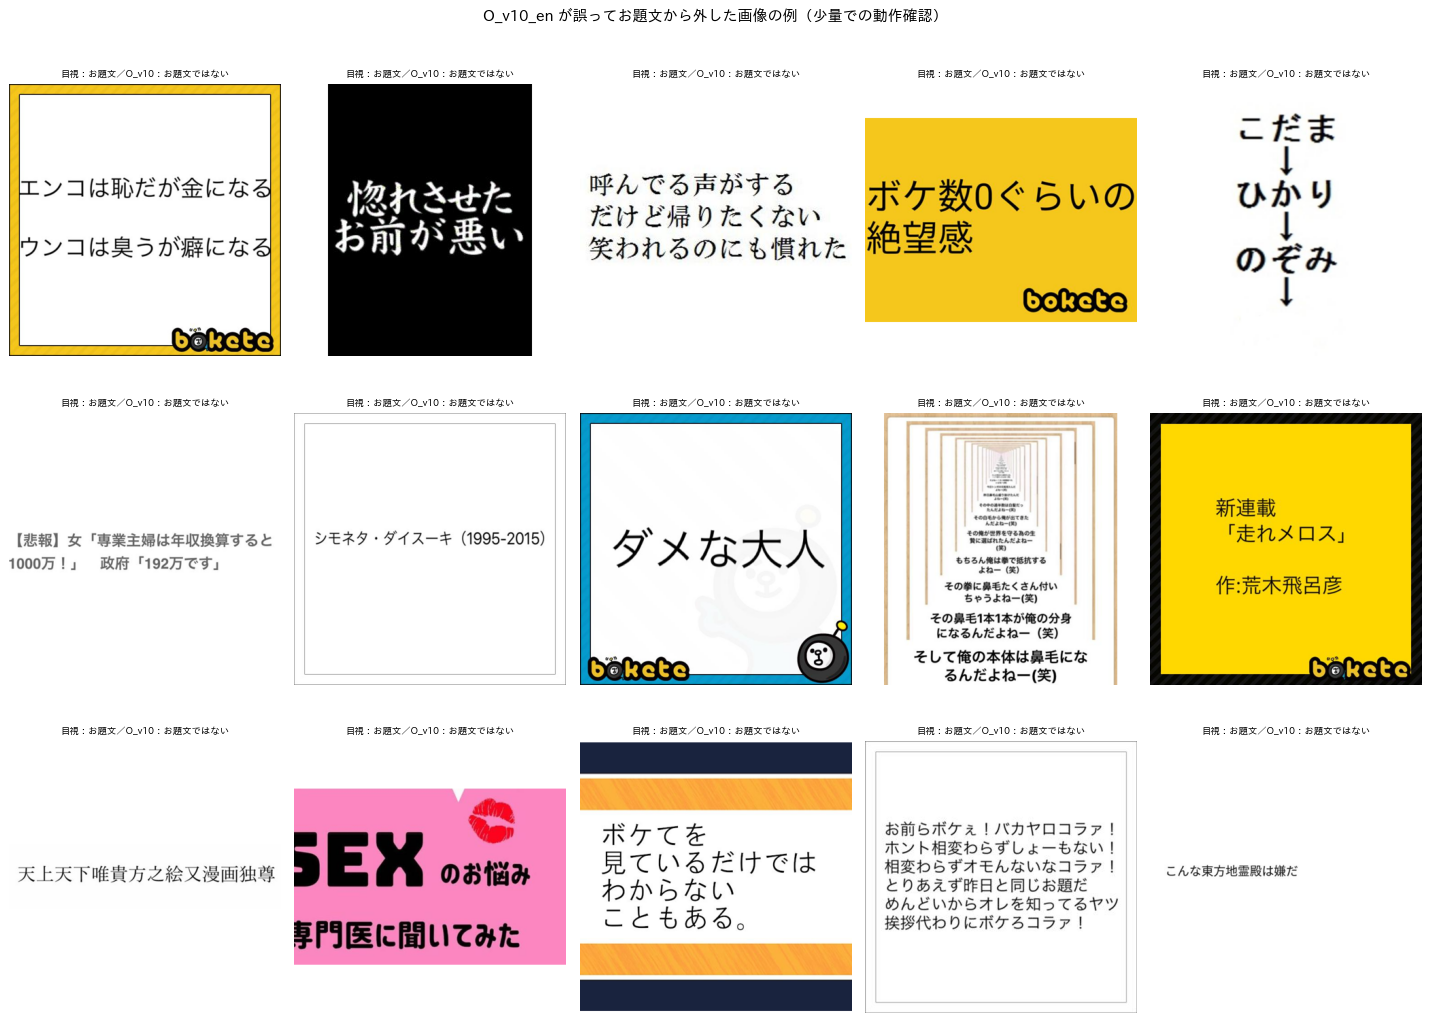
\includegraphics[width=0.8\textwidth]{figures/fig_o10_wrong.png}
    \caption{教師の構成の確認の質問が誤ってお題文から外した画像の例．画像の上に目視の形式と確認の質問の回答を示す}
    \label{fig_o10_wrong}
\end{figure*}

そこで，題目の句の典型的な型と，テンプレートや無地の背景に書かれた主題の文を真とする例として明示し，看板，報道の画面，ウェブの記事，歌詞，ゲームや漫画の台詞など文字が全て元の素材から来ている場合を偽とする例として明示した確認の質問を作成した．
実装の識別子は O\_v11\_en である．
この質問がお題文ではないと答えたのは9枚であり，アプリのエラー画面，ゲームの画面，報道の画面，看板などで，全て正しかった．
効果は全データの約0.05\%と小さいが，誤りは見つからなかったため，最終の構成ではこの質問を用いた．

なお，教師ラベルをこの質問で作り直した場合も比較したが，その教師ラベルで学習した生徒はお題文と予測する割合が実データで9.5\%と高くなり，全ての評価で劣った．
そのため，教師ラベルは表\ref{tab_questions}の構成のままとした．
ボケの書き出しによるカルタの取り消しも比較したが，生徒の予測では評価用データ全体で1枚しか変わらず，その1枚は正しいカルタであったため用いなかった．
教師ではこの規則がカルタの誤検出を減らしたが，生徒はカルタの誤検出が既に少ないためである．

\subsection{最終の構成の精度}
表\ref{tab_final_items}に，最終の構成の項目ごとの F1 を示す．
test は通常の評価用データの最終評価用の320枚，層別は実データの層別抽出の220枚での値，推定は(\ref{eq_ipw})による実際の分布での推定値である．

\begin{table}[t]
    \centering
    \caption{最終の構成の項目ごとの F1}
    \label{tab_final_items}
    \small
    \begin{tabular}{llccc}
        \toprule
        軸 & 項目 & test & 層別 & 推定 \\
        \midrule
        \multirow{4}{*}{形式} & カルタ & 0.88 & 1.00 & 1.00 \\
         & 穴埋め & 0.93 & 0.98 & 0.94 \\
         & お題文 & 0.89 & 0.86 & 0.87 \\
         & 通常 & 0.96 & 0.97 & 0.97 \\
        \midrule
        \multirow{2}{*}{属性} & 空欄あり & 0.94 & 0.98 & 0.95 \\
         & 文字あり & 0.97 & 0.97 & 0.97 \\
        \midrule
        \multirow{7}{*}{媒体} & 写真 & 0.97 & 0.96 & 0.98 \\
         & アニメ & 0.89 & 0.96 & 0.88 \\
         & ゲーム & 0.89 & 0.91 & 0.90 \\
         & マンガ & 0.91 & 0.98 & 0.99 \\
         & テキストグラフィック & 0.95 & 0.90 & 0.92 \\
         & 絵画 & 1.00 & 0.79 & 0.46 \\
         & イラスト & 0.78 & 0.73 & 0.82 \\
        \bottomrule
    \end{tabular}
\end{table}

最終の構成は，通常の評価用データの test で3軸の平均 0.919，少ない区分の評価用データの test でゲーム，絵画，カルタの F1 の平均 0.888，実データの全項目一致の推定値 0.838 を達成した．
埋め込みの MLP 単体では，それぞれ 0.886，0.845，0.797 であった．
test のゲームは5枚，絵画は3枚のみであり，F1 の値は不安定である．
絵画の推定値 0.46 も，実データの目視ラベルに絵画が15枚しかなく，重みの大きい1枚から2枚の誤りで大きく動く．
絵画の精度は，少ない区分の評価用データでの F1 0.84 で見るのが適切である．
最も低い項目はイラストであり，アニメ風の一枚絵，ゲームの絵，絵本の挿絵との境界が曖昧で，目視でも判断が分かれた．

\subsection{精度の推移}
表\ref{tab_progress}に，研究の各段階の代表的な構成の精度を示す．
定義が変わると評価用ラベルも付け直しているため，異なる段階の数値は厳密には比較できないが，段階ごとの改善の傾向を示す．

\begin{table}[t]
    \centering
    \caption{研究の各段階の代表的な生徒の精度}
    \label{tab_progress}
    \small
    \begin{tabular}{>{\raggedright\arraybackslash}p{0.5\linewidth}>{\raggedright\arraybackslash}p{0.38\linewidth}}
        \toprule
        段階と生徒 & 精度 \\
        \midrule
        初期の7クラス，線形プローブ & 正解率 0.913 \\
        第1版の4軸，MLP & 4軸の平均 0.778 \\
        第2版の3軸，微調整，追加ありと重み & test の3軸の平均 0.812 \\
        第2版，絵画の質問を加えた教師，MLP & test の3軸の平均 0.822 \\
        第3版，MLP，追加あり & test の3軸の平均 0.897 \\
        第4版，MLP，追加あり & 全項目一致の推定値 0.802 \\
        第4版，最終の構成 & test の3軸の平均 0.919，全項目一致の推定値 0.838 \\
        \bottomrule
    \end{tabular}
\end{table}

\subsection{処理時間}
予測の段階は，GPU での SigLIP2-so400m の計算が律速であり，画像の読み込みのプロセス数を増やしても速度は GPU のみの速度である毎秒約205枚に近い値にとどまった．
無作為の2万枚での予測の速度は毎秒約150枚，確認の質問の速度は毎秒約22枚であった．
処理時間を優先する場合は，確認の質問を省くと全項目一致の推定値をほぼ保ったまま確認の段階を省け，微調整した SigLIP2-B のみを用いると全件を約2.5時間で処理できるが，全項目一致の推定値は 0.795 に下がる．
